% -*- TeX -*- -*- UK -*- -*- Soft -*-"

\chapter{Setting up WinEdt}

\section{Install WinEdt}
\label{sec:installwinedt}
This document assumes that WinEdt v.10.0 is installed.

After you changed an ini file, the changes can be immediately be made available by clicking on the load button:

\centerline{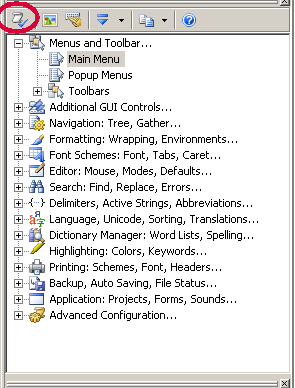
\includegraphics[bb= 0 0 295 388, width=0.4\textwidth]{eps/loadini.png}}

After you make changes to a particular script you should use the Load Command (the first button in the Option Interface Toolbar) to make the changes effective immediately. It is not necessary to restart WinEdt. In fact, no scripts are loaded at startup: the compiled raw data is stored in WinEdt.dnt (Do Not Touch). This reduces the startup time and reduces the likelihood of error messages during startup.


I am not quite sure how to activate the changes for the next time you start WinEdt.  It seems that exporting to WinEdt.dnt have the effect of saving the changes to that these are working next time you load WinEdt.

\section{Viewer Setup}

Yap seemed to fail on my WinEdt install.

MikTeX provides a DVI viewer, called YAP that integrates well with WinEdt. If properly set up, WinEdt and YAP are synchronised. When you run the \LaTeX{} compiler, YAP will open at the location of the cursor in the WinEdt file. When you double click in the YAP window, the text cursor in WinEdt will move to the corresponding location.

The Yap binary is located in the MikTeX bin file, on my PC at
\url{C:\Program Files\MiKTeX 2.9\miktex\bin\x64}

$<$Options$>$$<$Execution Modes$>$, select 'LaTeX'. If not set, set 'Wait for execution to finish' and select the 'Start Viewer' and 'Forward Search' boxes. The 'Start Viewer' selection will start the viewer after completion of the compilation process, and the 'Forward Search' selection will move a small, round, cursor to the location in the DVI viewer, where the cursor is in the LaTeX document (when it makes sense).

Other viewers can be started in a similar manner, just select the appropriate compiler in the left-hand box, and set 'Start Viewer' in the next box.


\centerline{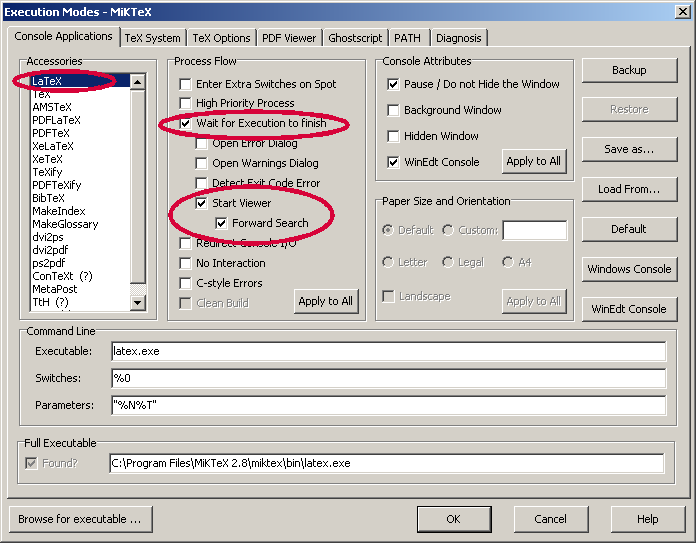
\includegraphics[bb= 0 0 696 543, width=\textwidth]{eps/StartViewer.png}}



In YAP go to  $<$View$>$$<$Options$>$$<$Inverse Search$>$, select WinEdt, if not yet selected. If option 'WInEdt' does not show in the dropdown box,  you have to enter the path to the application in the text box at the bottom of the dialog box.  On my installation, the entry is	\\
{\small \verb+"C:\Program Files\WinEdt Team\WinEdt 10\winedt.exe" "[Open(|%f|);SelPar(%l,8)]"+}

\centerline{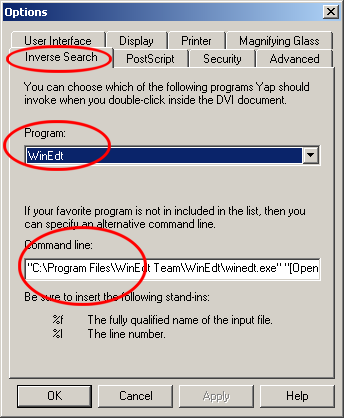
\includegraphics[bb= 0 0 344 416, width=.6\textwidth]{eps/yapinverse.png}}




These PDF viewers are currently available on my PC:
\begin{lstlisting}
C:\Program Files\Tracker Software\PDF Viewer\PDFXCview.exe
C:\Program Files\PDF Architect 7\architect.exe
C:\Users\nwillers\AppData\Local\SumatraPDF\SumatraPDF.exe
\end{lstlisting}


\section{Enabling Active Strings for  begin-end Pair}
It seems that the default settings are acceptable, no edit required. If you do need to change anything, go to
$<$Options$>$$<$Options Interface$>$$<$Delimiters, Active Strings, ...$>$$<$Active Strings$>$, edit the macro file just opened to enable \verb+"\begin{?}}"+. It might already be activated. Edit as required and save when done.

\centerline{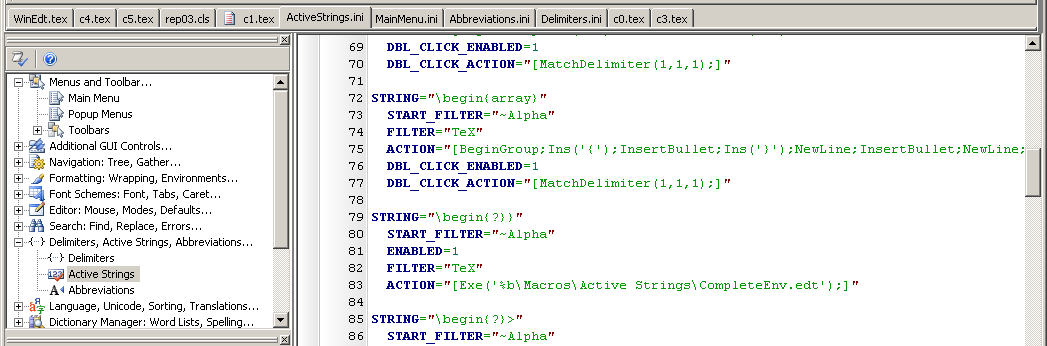
\includegraphics[bb= 0 0 1047 346, width=\textwidth]{eps/ASbegin.png}}

%It seems in WinEdt9, that you must type \verb"\begin{enumerate}}", i.e. with an extra \verb"}" to %activate the active string.


\section{Setting up the Dictionary}
$<$Options$>$$<$Options Interface$>$$<$Dictionary Manager:....$>$$<$Word Lists (.)...$>$, edit the macro file just opened.  You enable or disable
sub-dictionaries according to your requirement.


If you want both the UK and US English dictionaries, keep all of the below dictionaries on. You can then select the language on a per-file basis.
Use embedded emacs-style mode and submode commands as the first line of each file. For example, use\\
\verb"% -*- TeX -*- -*- US -*- -*- Soft -*-" for US spelling, or\\
\verb"% -*- TeX -*- -*- UK -*- -*- Soft -*-" for UK spelling in the tex file.\\
For more information search the WinEdt documentation for ``modes and submodes''.\\
See also
\begin{lstlisting}
\url{https://www.gnu.org/software/emacs/manual/html_node/emacs/Specifying-File-Variables.html}
\url{https://www.gnu.org/software/emacs/manual/html_node/emacs/Choosing-Modes.html}
\end{lstlisting}


If you require only UK English, as in in South Africa, select:\\
\textbf{Enable the following dictionaries:} User (Addon), EDT, LaTeX, WinEdt, English (common),  English (colour),  English (labelled),  English (centre), English (ise),  English  (yse).\\
\textbf{Disable the following dictionaries:}  English (Small), English (color), English (labeled), English (center), English (ize), English (yze).
Save the file when done.

\centerline{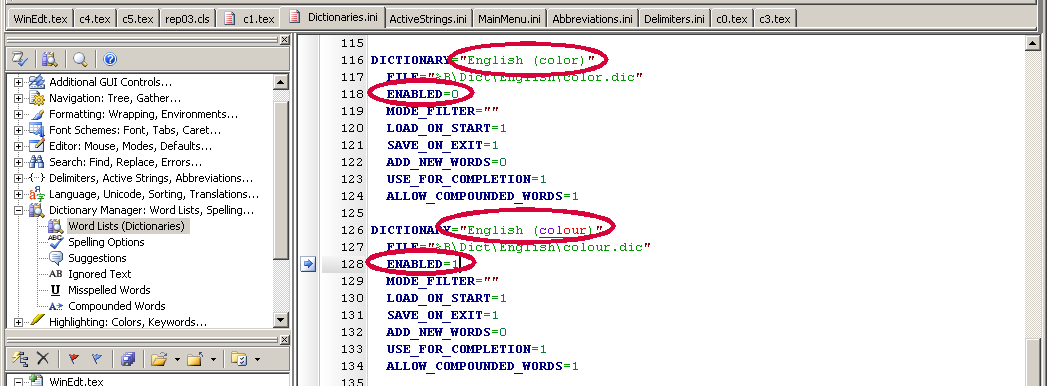
\includegraphics[bb= 0 0 1047 386, width=\textwidth]{eps/dictionary.png}}



\section{TeX Symbols GUI}

Activate the TeX Symbols GUI by clicking on the $\Sigma$-on-the grid symbol.

\centerline{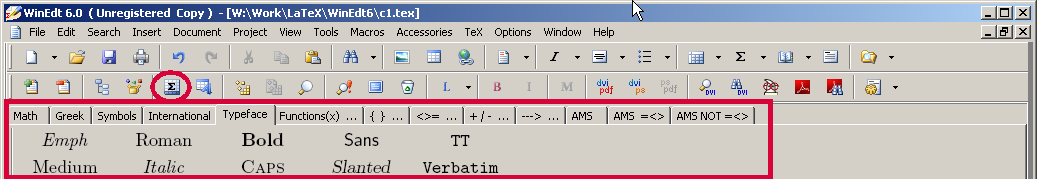
\includegraphics[bb= 0 0 1037 179,width=\textwidth]{eps/texsymbolsgiu.png}}



\section{Keep Whitespace at EOF and EOL}

$<$Options$>$$<$Options Interface$>$$<$Editor: Mouse, Modes,...$>$$<$Defaults$>$, edit the macro file just opened. Scroll down to 'Trim Spaces' and 'Trim lines' and disable these two (make the values 0) --- this is stop WinEdt from removing spaces at the end of lines and files.

\centerline{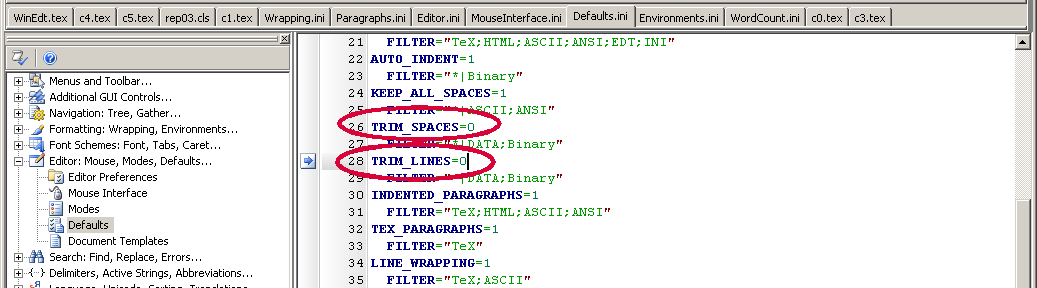
\includegraphics[bb= 0 0 1037 288,width=\textwidth]{eps/trimeoleof.png}}


\section{Set Text Wrapping and Text Width}

$<$Options$>$$<$Options Interface$>$$<$Formatting, Wrapping, Environments....$>$$<$Wrapping$>$, edit the macro file just opened.
Switch on or off if required and set the right margin. Defaults work fine in WinEdt 10.

\centerline{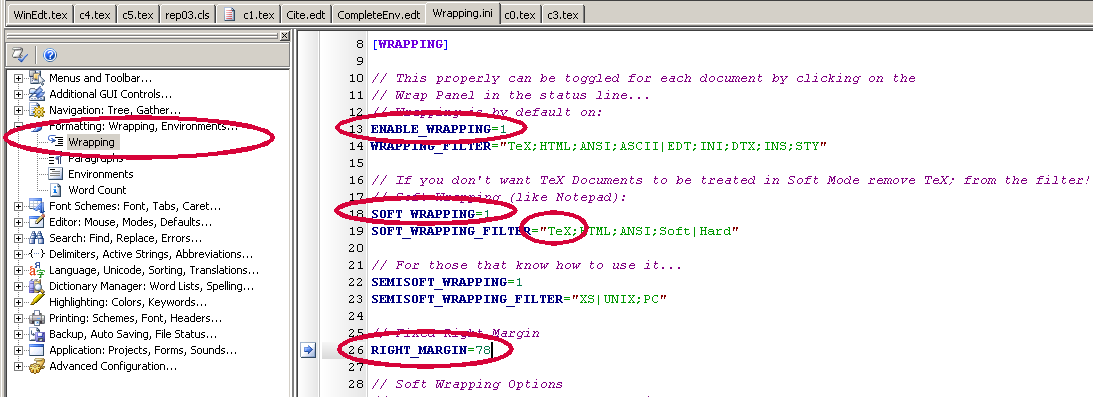
\includegraphics[bb= 0 0 1093 397,width=\textwidth]{eps/wrapping.png}}

\section{Add a Table-Paste Macro to a Menu}
\label{sec:addpastetable}

$<$Options$>$$<$Options Interface$>$$<$Menus and Toolbar$>$$<$Main Menu$>$, edit the macro file just opened. Add the text shown below at the indicated location just before the \lstinline{END="&Macros"} line.


\centerline{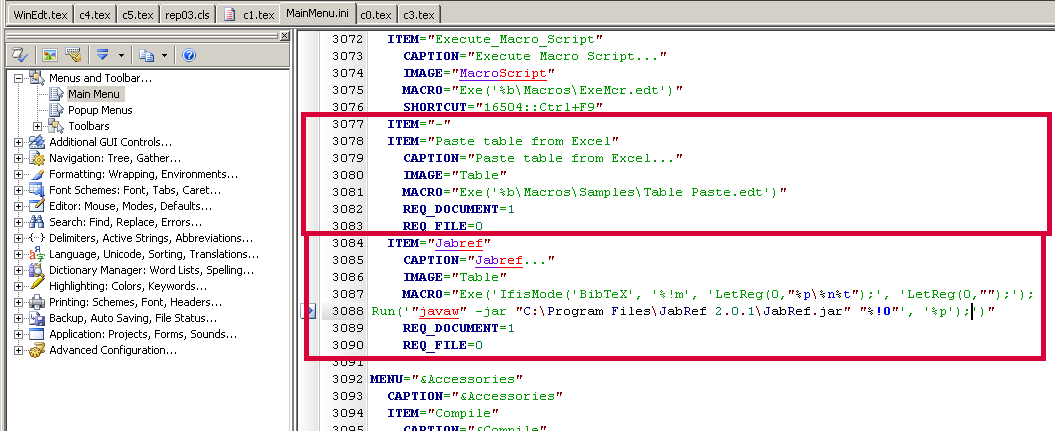
\includegraphics[bb= 0 0 1055 431,width=\textwidth]{eps/AddExcelTable.png}}

This picture does not shown the \lstinline{END="&Macros"} line It is required).

The picture above shows intalling JabRef, this is optional if installed.

\begin{lstlisting}[label=MacropastetableExcel,caption=Macro to paste table from Excel]
    ITEM="Paste table from Excel"
    CAPTION="Paste table from Excel..."
    IMAGE="Table"
    MACRO="Exe('%b\Macros\Samples\Table Paste.edt')"
    REQ_DOCUMENT=1
    REQ_FILE=0
\end{lstlisting}

Copy and paste [best to do this from the LaTeX source file] the text in Listing~\ref{MacropastetableExcel}. If it does not work,  check the MACRO line:  take care to use the upquote (\verb+'+,  next to the Enter key) and not the curly quote (').

If does not already exists: copy the following file (\lstinline{Table Paste.edt}) from the repo \lstinline{files} folder  (copy all three edt files)
 to the
\lstinline{C:/Program Files/WinEdt Team/WinEdt 10/Macros/Samples} or\\
\lstinline{C:/Users/nwillers/WinEdt Team/WinEdt 10/Macros/Samples}
folder.

\begin{lstlisting}
    // %-*- ASCII -*- -*- EDT -*-
    //
    // Paste Table and covert it to LaTeX format:
    //  Tab  -> &Tab
    //  EOLN -> \\EOLN

      Requires(20010317);  // Requires WinEdt 5 Build 20010317 (or later)

      CopyFromClipboard(0);  // Get the Clipboard Text Data (eg. Excel)

      // Convert Tab to &Tab
      LetRegNum(2, -2);
      Loop(!|>
        FindInString("%!0", "$[#9]$", 1,2, 1011, %!2+2);>
        IfOK(!'ReplaceInString("%!0", "&\&9;", %!1, %!2, 1, 0);',!'Stop;')|);

      // Convert EOLN to \\EOLN
      LetRegNum(2, -3);
      Loop(!|>
        FindInString("%!0", ">", 1,2, 1011, %!2+3);>
        IfOK(!'ReplaceInString("%!0", "\\\\>", %!1, %!2, 1, 0);',!'Stop;')|);

      InsText("%!0"); // Insert with no wrapping

    End;

    // WinEdt also has a Block/ Column mode selection that can come
    // handy when manipulating aligned tables...
\end{lstlisting}




\section{Add a Back Slash to Forward Slash Macro to a Menu}
\label{sec:bsfs}

$<$Options$>$$<$Options Interface$>$$<$Menus and Toolbar$>$$<$Main Menu$>$

Search down for the entry labelled \lstinline{MENU="&Accessories"}.
In the section just before Accessories, add the following:
\begin{lstlisting}
    ITEM="Backslash to Forward"
    CAPTION="Backslash to Forward..."
    IMAGE="Table"
    MACRO="Exe('%b\Macros\Samples\bstofs.edt')"
    REQ_DOCUMENT=1
    REQ_FILE=0
\end{lstlisting}
just before the \lstinline{END="&Macros"} line.

Add the file (\lstinline{bstofs.edt}) with the following contents to
\lstinline{C:/Program Files/WinEdt Team/WinEdt 10/Macros/Samples/bstofs.edt}

\begin{lstlisting}
SetFindStr("\");
SetReplaceStr("/");
SetSearchCaseSensitive(0);
SetSearchRelaxed(0);
SetSearchWholeWords(0);
SetSearchInline(0);
SetRegEx(0);
SetSearchSelected;
SetSearchCyclic(0);
SetSearchForward(1);
SetSearchEntire(0);
SetReplaceRespectCaps(1);
SetReplacePrompt(0);
SearchReset;
ReplaceAll;
// ReplaceDialog;
\end{lstlisting}


\section{Disable Synctex}

In WinEdt10 the default settings for LaTeX is to compile with option -synctex=-1 and, in WinEdt5.6, the default settings for LaTeX is without the -synctex option.
However, MiKTeX does not support the synctex option for filenames with spaces.

The solution is to open WinEdt and uncheck 'Use -synctex switch' in $<$Options$>$ $<$Execution Modes$>$$<$PDF Viewer$>$.

\centerline{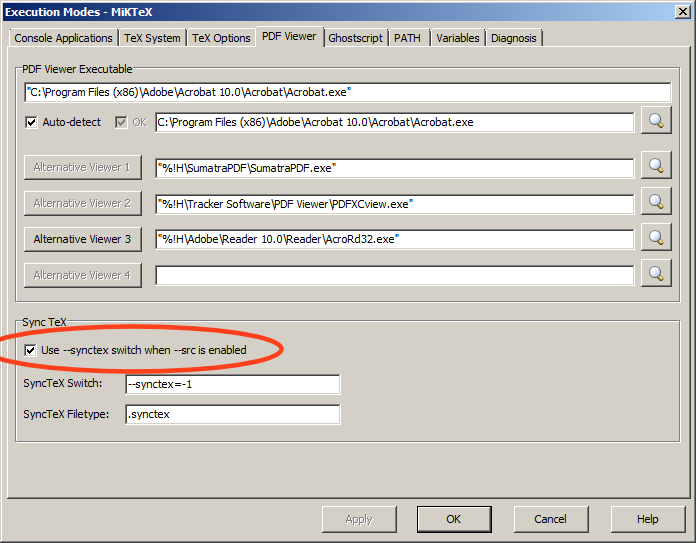
\includegraphics[bb= 0 0 696 543,width=0.8\textwidth]{eps/synctex.png}}

In the latest installs on Windows 7 it seems that this is no longer required; there can be spaces now. Experiment and find the best solution.


\section{Disable Autosaving and Backup}

Disable auto-saving and keeping backup files, by $<$Options$>$ $<$Preferences$>$$<$Backup$>$ and unchecking the relevant boxes.

\centerline{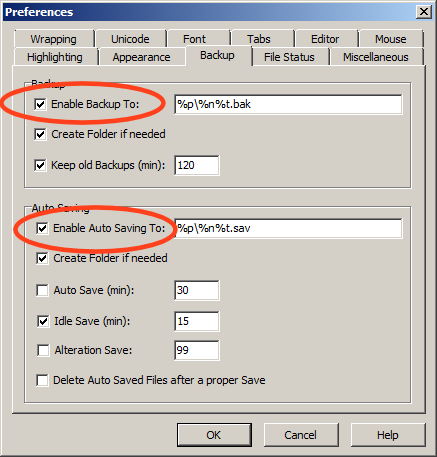
\includegraphics[bb= 0 0 437 457,width=0.6\textwidth]{pic/savingback.png}}




\section{Adding to TeX Symbols }
You may want to add new buttons to the \TeX\ symbols Typeface GUI.
Rename the existing \url{Typeface.bmp} to \url{Typeface-old.bmp} in the following folders, and then add the new (bigger) \url{Typeface.bmp} from the repo \url{files} folder to the same GUI folders. Copy the appropriately sized bitmap according to the folder structure.


\centerline{
\includegraphics[bb= 0 0 999 88, width=\textwidth]{pic/Typeface.png}}

\noindent
\url{C:\Program Files\WinEdt Team\WinEdt 10\Bitmaps\Gui}\\
\url{C:\Program Files\WinEdt Team\WinEdt 10\Bitmaps\Gui125}\\
\url{C:\Program Files\WinEdt Team\WinEdt 10\Bitmaps\Gui200}\\
or (replace with your user name)\\
\url{C:\Users\nwillers\WinEdt Team\WinEdt 10\Bitmaps\Gui}\\
\url{C:\Users\nwillers\WinEdt Team\WinEdt 10\Bitmaps\Gui125}\\
\url{C:\Users\nwillers\WinEdt Team\WinEdt 10\Bitmaps\Gui200}\\



$<$Options$>$$<$Options Interface$>$$<$Additional GUI Controls...$>$$<$TeX Symbols$>$, edit the macro file just opened. Locate this section corresponding to the Typeface part of the GUI and replace the entire block with the following block:

\begin{lstlisting}
  PAGE="Typeface"
  CAPTION="Typeface"
  CONFIG_FILTER=""
  MODE_FILTER=""
  GROUP="Typeface.bmp"
    TOP=0
    SPACE=0
    ROWS=2
    COLUMNS=10
    WIDTH=111
    HEIGHT=32
    ITEM="\emph{...}"
      MACRO="Exe('%b\Macros\Fonts\Emphasize.edt');"
    ITEM="\textrm{...}"
      MACRO="Exe('%b\Macros\Fonts\Roman.edt');"
    ITEM="\textbf{...}"
      MACRO="Exe('%b\Macros\Fonts\Bold.edt');"
    ITEM="\textsf{...}"
      MACRO="Exe('%b\Macros\Fonts\SansSerif.edt');"
    ITEM="\texttt{...}"
      MACRO="Exe('%b\Macros\Fonts\TypeWriter.edt');"
    ITEM="\url{...}"
        MACRO="Exe('%b\Macros\Fonts\FormatURL.edt');"
    ITEM="\inline{...}"
        MACRO="Exe('%b\Macros\Fonts\FormatInline.edt');"
    ITEM="\index{...}"
        MACRO="Exe('%b\Macros\Fonts\FormatIndex.edt');"
    ITEM="\textsup{...}"
        MACRO="Exe('%b\Macros\Fonts\Formattextsuperscript.edt');"
    ITEM="\sout{...}"
        MACRO="Exe('%b\Macros\Fonts\FormatSout.edt');"
    ITEM="\textmd{...}"
      MACRO="Exe('%b\Macros\Fonts\Medium.edt');"
    ITEM="\textit{...}"
      MACRO="Exe('%b\Macros\Fonts\Italic.edt');"
    ITEM="\textsc{...}"
      MACRO="Exe('%b\Macros\Fonts\SmallCaps.edt');"
    ITEM="\textsl{...}"
      MACRO="Exe('%b\Macros\Fonts\Slanted.edt');"
    ITEM="\verb""..."""
      MACRO="Exe('%b\Macros\Fonts\Verbatim.edt');"
    ITEM="\TBC{...}"
        MACRO="Exe('%b\Macros\Fonts\FormatTBB.edt');"
    ITEM="\scmnd{...}"
        MACRO="Exe('%b\Macros\Fonts\FormatScmnd.edt');"
    ITEM="\nomen{...}"
        MACRO="Exe('%b\Macros\Fonts\FormatNomenclature.edt');"
    ITEM="\textsub{...}"
        MACRO="Exe('%b\Macros\Fonts\Formattextsubscript.edt');"
    ITEM="\textcolor{...}"
        MACRO="Exe('%b\Macros\Fonts\FormatTextColor.edt');"
\end{lstlisting}

If required, you can add even more new buttons to the current image, but it is somewhat tricky. Take care that you keep the new buttons the same size. Also add the code for the new buttons as shown above.

It seems that you specify the number of rows and columns in the GUI and also the width and height of each button (which do not quite match up to the image size).  Change the number of columns and insert the new button's code in the appropriate location in the list (e.g. url and TBC above).

After you have edited the above ini file, save the file and load the changes as shown in Section~\ref{sec:installwinedt}.

Either copy the \lstinline{edt} files from the repo folder \lstinline{files/Macros/Fonts} to the installation folder
\lstinline{Macros/Fonts}. Alternatively reconstruct the files from the following text. Create the appropriate scripts, with the contents below, and save these in \url{Macros/Fonts/}:


\begin{lstlisting}
--- old 555x88 96 ppi  new 999x88 72 ppi

125 old  520x56 168ppi new

200 old  800x88 168ppi new  1798x88 72 ppi
\end{lstlisting}





File \texttt{FormatIndex.edt}
\begin{lstlisting}
// -*- ASCII:EDT -*-

BeginGroup;
IfSel('0','=',>
      'SelWord(1);>
       IfSel(''0'',''='',>
             ''Ins("\index{}");>
               CharLeft;'',>
             ''InsLabel("\index","{","}")'');',>
      'InsLabel("\index","{","}");');
EndGroup;
End;
\end{lstlisting}


Filename \texttt{FormatInline.edt}
\begin{lstlisting}
// -*- ASCII:EDT -*-

BeginGroup;
IfSel('0','=',>
      'SelWord(1);>
       IfSel(''0'',''='',>
             ''Ins("\lstinline{}");>
               CharLeft;'',>
             ''InsLabel("\lstinline","{","}")'');',>
      'InsLabel("\lstinline","{","}");');
EndGroup;
End;
\end{lstlisting}

Filename \texttt{FormatNomenclature.edt}
\begin{lstlisting}
// -*- ASCII:EDT -*-

  BeginGroup;
IfSel('0','=',>
      'SelWord(1);>
       IfSel(''0'',''='',>
             ''Ins("\nomenclature{}{}");>
               CharLeft;'',>
             ''InsLabel("\nomenclature","{","}{}")'');',>
       'InsLabel("\nomenclature","{","}{}");');>
EndGroup;
End;
\end{lstlisting}

Filename \texttt{FormatScmnd.edt}
\begin{lstlisting}
// -*- ASCII:EDT -*-

BeginGroup;
IfSel('0','=',>
      'SelWord(1);>
       IfSel(''0'',''='',>
             ''Ins("\scmnd{}");>
               CharLeft;'',>
             ''InsLabel("\scmnd","{","}")'');',>
      'InsLabel("\scmnd","{","}");');
EndGroup;
End;
\end{lstlisting}

File \texttt{FormatTBC.edt}
\begin{lstlisting}
// -*- ASCII:EDT -*-

BeginGroup;
IfSel('0','=',>
      'SelWord(1);>
       IfSel(''0'',''='',>
             ''Ins("\TBC{}");>
               CharLeft;'',>
             ''InsLabel("\TBC","{","}")'');',>
      'InsLabel("\TBC","{","}");');
EndGroup;
End;
\end{lstlisting}


Filename \texttt{Formattextsubscript.edt}
\begin{lstlisting}
  // -*- ASCII:EDT -*-

  BeginGroup;
  IfSel('0','=',>
        'SelWord(1);>
         IfSel(''0'',''='',>
               ''Ins("\textsubscript{}");>
                 CharLeft;'',>
               ''InsLabel("\textsubscript","{","}")'');',>
        'InsLabel("\textsubscript","{","}");');
  EndGroup;
  End;
\end{lstlisting}


Filename \texttt{Formattextsuperscript.edt}
\begin{lstlisting}
  // -*- ASCII:EDT -*-

  BeginGroup;
  IfSel('0','=',>
        'SelWord(1);>
         IfSel(''0'',''='',>
               ''Ins("\textsuperscript{}");>
                 CharLeft;'',>
               ''InsLabel("\textsuperscript","{","}")'');',>
        'InsLabel("\textsuperscript","{","}");');
  EndGroup;
  End;
\end{lstlisting}

Filename \texttt{FormatURL.edt}
\begin{lstlisting}
// -*- ASCII:EDT -*-

BeginGroup;
IfSel('0','=',>
      'SelWord(1);>
       IfSel(''0'',''='',>
             ''Ins("\url{}");>
               CharLeft;'',>
             ''InsLabel("\url","{","}")'');',>
      'InsLabel("\url","{","}");');
EndGroup;
End;
\end{lstlisting}


If you are using nomenclature download and install the following macro:\\
\url{http://www.winedt.org/config/menus/Nomenclature.html}

\section{Adding New Environments to Insert Menu}

You may want to add new menu items to the existing menu system.

$<$Options$>$$<$Options Interface$>$$<$Menu and Toolbar...$>$$<$Main Menu$>$, edit the macro file just opened. Locate this section corresponding to the submenu for environment insertions:

\begin{lstlisting}
  SUBMENU="Environments>"
      CAPTION="&Environments"
      CONFIG_FILTER="Default;MiKTeX;TeX Live"
      IMAGE="Env"
      REQ_DOCUMENT=1
\end{lstlisting}

and insert the code to create new listings at the end, just before   \verb+END="Environments>"+

\begin{lstlisting}
    ITEM="-"
     ITEM="lstlisting"
      CAPTION="&lstlisting"
      MACRO="LetReg(9,'lstlisting');LetReg(8);Exe('%b\Menus\Insert\Env.edt');"
      REQ_DOCUMENT=1
    ITEM="-"
\end{lstlisting}

After you have edited the above ini file, save the file and load the changes as shown in Section~\ref{sec:installwinedt}.

Then copy the file \verb+env.tab+  from the repo \lstinline{files} folder to
\lstinline{Menus/Insert}

\section{Change the Default Insert Templates}

WinEdt keeps its templates for inserted text in the following directory:\\
\verb+C:\Program Files\WinEdt Team\WinEdt 10\Templates\LaTeX+.\\
Modify any of the templates in this directory to suit your needs.  The text insertion is available under the 'Insert' menu entry.


\section{Add a Macro to Activate Jabref}

If you are using Jabref:

Using the same procedure as described in Section~\ref{sec:addpastetable}, create a new menu entry and paste the following code into the 'Macro' box (all on one line):

{\footnotesize
\begin{verbatim}
[IfisMode('BibTeX', '%!m', 'LetReg(0,"%p\%n%t");', 'LetReg(0,"");');
Run('"javaw" -jar "C:\Program Files\JabRef 2.0.1\JabRef.jar" "%!0"', '%p');]
\end{verbatim}
}

where the reference to Jabref must be to the jar file, as installed on your PC.

{\footnotesize
\begin{verbatim}
  ITEM="Jabref"
    CAPTION="Jabref..."
    IMAGE="Table"
    MACRO="Exe('IfisMode('BibTeX', '%!m', 'LetReg(0,"%p\%n%t");', 'LetReg(0,"");');
    Run('"javaw" -jar "C:\Program Files (x86)\JabRef\JabRef-2.10.jar" "%!0"', '%p');')"
    REQ_DOCUMENT=1
    REQ_FILE=0
\end{verbatim}
}


\section{Enable File Update Warnings}

Sometimes you update a file externally (e.g. subversion updates the file version) and you want to be warned of this event.

$<$Options$>$$<$Options Interface$>$$<$Editor: Mouse, Modes.....$>$$<$Defaults$>$, edit the macro file just opened. Confirm that the values are set to 1 as  shown below at the indicated location.

\centerline{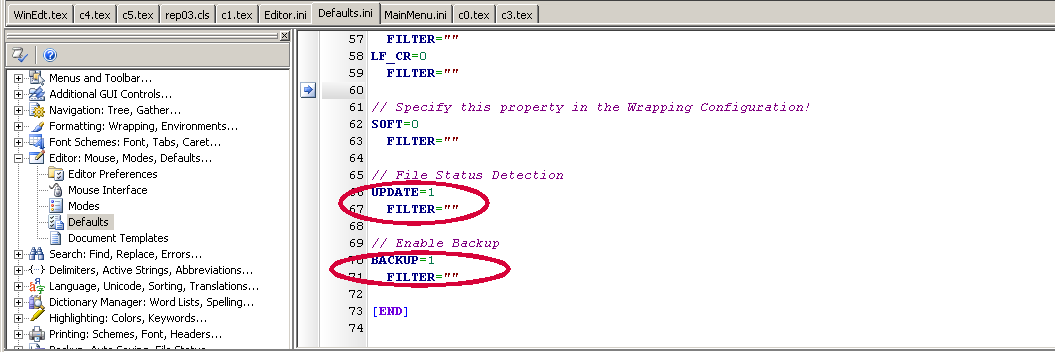
\includegraphics[bb= 0 0 1055 352,width=\textwidth]{eps/updatedrives.png}}


\section{Add files to 'Erase working file' GUI}

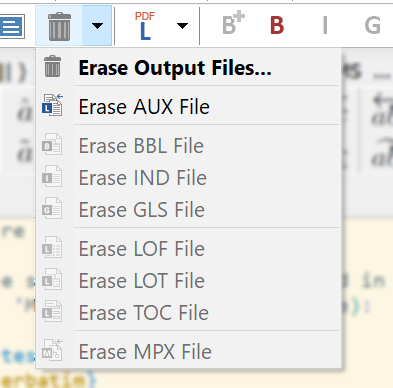
\includegraphics[width=50mm]{pic/recycle-clutter.png}

The recycle bin icon provides a convenient way to remove clutter from the working folder.
The GUI is defined by the file \\
\lstinline{%USER%\AppData\Roaming\WinEdt Team\WinEdt 10\Exec//Erase Working Files.edt}
or try this one\\
\lstinline{WinEdt Team/WinEdt 10/Exec/Erase Working Files.edt}, which can be adapted for your needs.

In the following changed file the items to remove mw files is added and all sync files is set to be ticked by default:

\begin{lstlisting}
// Erase Working Files Interface
// =============================
//
// Modify the default in this value (if needed):
//
//      AddFileItem(Enabled: 0..1, "Description","Filename","Mode Filter");
//
// Use the macro EraseWorkingFiles to invoke a GUI for this interface:
//
//      EraseWorkingFiles("Folder List;", "Caption", Subfolders: -1..1, Invisible: 0..1);

    ClearFileItems;

    AddFileItem(0,"PDF File","%N.pdf","TeX");
    AddFileItem(1,"SYNC File","*.synctex.*","TeX");

    AddFileItem(1,"DVI File","%N.dvi","TeX");
    AddFileItem(1,"PS  File","%N.ps","TeX");

    AddFileItem(1,"LOG Files","*.log","");
    AddFileItem(1,"AUX Files","*.aux","TeX");
    AddFileItem(1,"BBL Files","*.bbl","TeX");
    AddFileItem(1,"BIT Files","*.bit","TeX");
    AddFileItem(1,"BLG Files","*.blg","TeX");
    AddFileItem(1,"BCF Files","*.bcf","TeX");
    AddFileItem(1,"BRF Files","*.brf","TeX");
    AddFileItem(1,"IDX Files","*.idx","TeX");
    AddFileItem(1,"IND Files","*.ind","TeX");
    AddFileItem(1,"ILG Files","*.ilg","TeX");
    AddFileItem(1,"GLO Files","*.glo","TeX");
    AddFileItem(1,"GLS Files","*.gls","TeX");
    AddFileItem(1,"GLG Files","*.glg","TeX");
    AddFileItem(1,"LOF Files","*.lof","TeX");
    AddFileItem(1,"LOT Files","*.lot","TeX");
    AddFileItem(1,"TOC Files","*.toc","TeX");
    AddFileItem(1,"OUT Files","*.out","TeX");
    AddFileItem(1,"TBB Files","*.tbb","TeX");
    AddFileItem(1,"TBC Files","*.tbc","TeX");
    AddFileItem(1,"x.pdf Files","*x.pdf","TeX");
    AddFileItem(1,"MW Files","*.mw","TeX");
    AddFileItem(1,"fdb_latexmk Files","*.fdb_latexmk","TeX");

    AddFileItem(1,"fls Files","*.fls","TeX");
    AddFileItem(1,"glsdefs Files","*.glsdefs","TeX");
    AddFileItem(1,"glx Files","*.glx","TeX");
    AddFileItem(1,"gxg Files","*.gxg","TeX");
    AddFileItem(1,"gxs Files","*.gxs","TeX");
    AddFileItem(1,"ist Files","*.ist","TeX");
    AddFileItem(1,"loa Files","*.loa","TeX");
    AddFileItem(1,"lol Files","*.lol","TeX");
    AddFileItem(1,"maf Files","*.maf","TeX");
    AddFileItem(1,"mtc Files","*.mtc","TeX");
    AddFileItem(1,"pag Files","*.pag","TeX");
    AddFileItem(1,".run.xml Files","*.run.xml","TeX");
    AddFileItem(1,"snm Files","*.snm","TeX");
    AddFileItem(1,"tdo Files","*.tdo","TeX");
    AddFileItem(1,"tns Files","*.tns","TeX");
    AddFileItem(1,"vtc Files","*.vtc","TeX");
    AddFileItem(1,"url Files","*.url","TeX");
    AddFileItem(1,"synctex Files","*.synctex","TeX");
    AddFileItem(1,"comment.cut","comment.cut","TeX");

    AddFileItem(1,"MPX Files","*.mpx","MetaPost");

    AddFileItem(1,"BAK Files","*.bak","");
    AddFileItem(1,"SAV Files","*.sav","");
    AddFileItem(1,"TMP Files","*.tmp","");
    AddFileItem(1,"MW Files","*.mw","TeX");



    AddFileItem(1,"TEMP Files","_temp.*","TeX");

    EraseWorkingFiles("%P;%O","Erase Output Files",0,0);

End;
\end{lstlisting}

\section{Enable Multiple Instances of WinEdt}

$<$Options$>$$<$Options Interface$>$$<$Application: Projects, Forms, ....$>$$<$Additional Preferences$>$, near line 62 set the value to 0:

\begin{lstlisting}
// Rather than disabling this option use -C command switch!
RUN_ONE_INSTANCE_ONLY=1
\end{lstlisting}

Or as suggested, leave this at 1 and just open an instance of WinEdt on the commandline with the following:

WinEdt -C="window title"

It is not clear why but some installations can open WinEdt without having the PATH setting to the executable.

\section{Colour Theme and Font}

To set a colour theme select from the
$<$Options$>$$<$Theme$>$$<$ menu.  If this does not work, experiment with \\
$<$Options$>$$<$Options Interface$>$$<$Highlighting, Colors ...$>$$<$Colors$>$. Scroll to \lstinline{Solarized Light} and uncomment the theme you require, and comment out all those not required.  Now it is a bit of a hit-and-miss using the menu options and selecting \lstinline{Default} from an empty list, to get the scheme to work.


Set the font to consolas, it reads easier than courier.

\section{Set Spelling Error Underline}

To increase the boldness of the spelling error underline select from the
$<$Options$>$$<$Options Interface$>$$<$Dictionary: Words Lists, Spelling...$>$$<$Missspelled words$>$. 


\begin{lstlisting}
[MISSPELLED_WORDS]
...
UNDERLINE_WEIGHT=+9 // -9=light .. 0=normal .. +9=heavy
...
BOLD=1
...
\end{lstlisting}


\section{LaTeXify}

\url{http://www.winedt.org/config/menus/LaTeXify.html}

This package adds a few items to the TeX menu, giving the user the chance to run an automated compilation by simply typing a shortcut or pressing a toolbar button.  Download and upzip, open \lstinline{Install.edt } in WnEdt. The run the macro  by choosing $<$Macros$>$ | $<$Execute Current Macro$>$.  You can launch your automated compilation from the TeX menu or the toolbar or typing one of the following shortcuts:

Biber (runs Biber) Shortcut: Ctrl+Alt+B\\
PDFLaTeXify (runs Biber and PDFTeXify with PDFLaTeX engine) Shortcut: Ctrl+Alt+P

\section{Executing Biber}

Install LaTeXify as described above. Biber should be available on the menu $<$ Tex$>$|$<$ Biber$>$.

Biber may however not be available as a button on the toolbar. Open
$<$Options$>$$<$Options Interface$>$$<$Menus and Toolbar$>$$<$Toolbar$>$, this should open \lstinline{toolbar.ini}.
Scroll down to near line 120, to the text the looks this this:

\begin{lstlisting}
// Alternatives:
// =============
//
// %%INCLUDE="ConfigEx\Toolbars\Toolbar1l.ini" // 1-row Toolbar (Large)
// %%INCLUDE="ConfigEx\Toolbars\Toolbar1s.ini" // 1-row Toolbar (Small)
// %%INCLUDE="ConfigEx\Toolbars\Toolbar1c.ini" // 1-row Toolbar (Custom)
// %%INCLUDE="ConfigEx\Toolbars\Toolbar2l.ini" // 2-row Toolbar (Large)
// %%INCLUDE="ConfigEx\Toolbars\Toolbar2s.ini" // 2-row Toolbar (Small)
// %%INCLUDE="ConfigEx\Toolbars\Toolbar2c.ini" // 2-row Toolbar (Custom)
// %%INCLUDE="ConfigEx\Toolbars\Toolbar5x.ini" // 2-row (WinEdt 5-style) Toolbar
\end{lstlisting}

Uncomment and double click on the line containing the toolbar you want to use, e.g.,  2-row Toolbar (Large).

\begin{lstlisting}
// Alternatives:
// =============
//
// %%INCLUDE="ConfigEx\Toolbars\Toolbar1l.ini" // 1-row Toolbar (Large)
// %%INCLUDE="ConfigEx\Toolbars\Toolbar1s.ini" // 1-row Toolbar (Small)
// %%INCLUDE="ConfigEx\Toolbars\Toolbar1c.ini" // 1-row Toolbar (Custom)
   %%INCLUDE="ConfigEx\Toolbars\Toolbar2l.ini" // 2-row Toolbar (Large)
// %%INCLUDE="ConfigEx\Toolbars\Toolbar2s.ini" // 2-row Toolbar (Small)
// %%INCLUDE="ConfigEx\Toolbars\Toolbar2c.ini" // 2-row Toolbar (Custom)
// %%INCLUDE="ConfigEx\Toolbars\Toolbar5x.ini" // 2-row (WinEdt 5-style) Toolbar
\end{lstlisting}

This will open \lstinline{Toolbar2l.ini}. Scroll down to the Bibtex entry near line 206.  Add a new biber button entry as follows, just before the BibTex entry.

\begin{lstlisting}
    MENU="-"
    MENU="XeLaTeX"
    MENU="XeTeX"
  BUTTON="|"
  BUTTON="Biber"
  BUTTON="BibTeX"
  BUTTON="Make_Index"
\end{lstlisting}

Now save the file and then run the command $<$Options$>$$<$Maintenance$>$$<$Rebuild All$>$.

If not yet selected, select the large 2-row toolbar in the menu
$<$Options$>$$<$Toolbar$>$$<$2-row large$>$ to select the newly-updated toolbar.  The biber button should now the visible.


\lstinline{https://tex.stackexchange.com/questions/316798/winedt-latexify-macro-install-fails-to-install-toolbar-buttons}

\section{See also}

\url{http://nakhmani.wordpress.com/2010/09/28/winedt-6-configuration/#more-44}
